%Енин Георгий ВТ-12
\section{ЭЛЕМЕНТЫ ДИСКРЕТНОГО ПРОГРАММИРОВАНИЯ}
\subsection{Некоторые задачи, приводящие к требованию целочисленности. Постановка задач дискретного программирования }
Среди практически важных задач отыскания условного экстремума линейной функции особое место занимают задачи с требованием целочисленности всех или части переменных. Они получили название задач целочисленного (частично целочисленного) программирования. Исторически первой задачей целочисленного типа явилась, опубликованная венгерским математиком Е. Эгервари в 1932 году, задача о назначении персонала.
\par\textit{Задача о назначениях.} Пусть требуется выполнить $n$ видов различных работ и имеется $n$ исполнителей (машин или людей) для их выполнения. Каждый исполнитель может использоваться на любой работе. Производительности исполнителей на различных работах, вообще говоря, различны. Обозначим через $c_{ij}$ производительность $i$-го исполнителя на $j$-ой работе. Задача заключается в таком распределении исполнителей по работам, при котором суммарная производительность максимальна.
\parПостроим математическую модель этой задачи. Для описания каждого варианта распределения исполнителей по работам введем переменные $x_{ij}$, относительно которых условимся, что $x_{ij}=1$, если $i$-й исполнитель назначен на $j$-ю работу, и $x_{ij}=0$ — в противном случае. Выбор варианта назначения исполнителей на работы равносилен приданию переменным $x_{ij}$ значений 0 или 1. При этом должны выполняться условия\\
$$\sum_{j=1}^n x_{ij} = 1, \; i = 1,2,...,n,$$
которые означают, что каждый исполнитель назначается на работу, а также условия
$$\sum_{i=1}^n x_{ij} = 1, \; j = 1,2,...,n,$$
которые означают, что каждая работа обеспечивается исполнителем. Суммарная производительность при данном варианте назначений выразится суммой
$$\sum_{i=1}^n \sum_{j=1}^n c_{ij}x_{ij}$$
\parТаким образом, получаем следующую математическую модель задачи
$$z = \sum_{i=1}^n \sum_{j=1}^n c_{ij}x_{ij}\rightarrow \textrm{max}$$
$$\sum_{j=1}^n x_{ij} = 1, \; i = 1,2,...,n,\; \sum_{i=1}^n x_{ij} = 1, \; j = 1,2,...,n,$$
$$	x_{ij} = \begin{cases}
		1\\
		0
	\end{cases}\hspace{-1em},\;\; i = 1,2,...,n,\;\;j = 1,2,...,n.
$$
\parПоследние из условий носят название условий булевости переменных $x_{ij}$, а задачи математического программирования с такими условиями называются задачами с булевыми переменными. Отметим, что замена условий булевости условиями неотрицательности переменных превращает нашу задачу в обычную закрытую транспортную задачу, если ее сформулировать как задачу на минимум. Если эту задачу решить методом потенциалов, то полученное решение автоматически будет удовлетворять условию булевости. Таким образом, в задаче о назначениях условия булевости переменных можно заменить условиями их неотрицательности. Отметим, что возможен открытый вариант задачи о назначениях, в котором количество исполнителей и видов работ не совпадают. С помощью введения фиктивных исполнителей или фиктивных видов работ эта задача сводится к такой же закрытой задаче, в которой производительности фиктивных пунктов полагаются равными нулю. При решении задачи некоторые исполнители могут оказаться без работы или некоторые виды работ — без исполнителей. При этом по-прежнему условия булевости можно заменить условиями неотрицательности.
\primer{
	Фирма объявила набор работников на две появившиеся вакансии. Были поданы заявления от трех претендентов, готовых занять каждую из двух вакансий. Предварительные испытания определили, что производительности претендентов на работе по каждой из двух вакансий задаются матрицей
	$$
		\begin{pmatrix}
			4 & 7 & 1\\
			5 & 3 & 6
		\end{pmatrix}.
	$$
}
\parТребуется так заполнить вакансии имеющимися претендентами, чтобы суммарная производительность принятых работников была максимальной. Предполагается, что каждая вакансия заполняется лишь одним претендентом, а каждый претендент может занять не более одной вакансии.
\parДля составления математической модели задачи введем такие переменные $x_{ij}$, что $x_{ij}=1$, если $i$-й исполнитель назначен на $j$-ю работу, и $x_{ij}=0$ — в противном случае. Получаем следующую задачу на максимум
$$
\begin{cases}
   x_{11} + x_{12} + x_{13} = 1,\\
   x_{21} + x_{22} + x_{23} = 1;
\end{cases}
\begin{cases}
	x_{11} + x_{21} \leq 1,\\
	x_{12} + x_{22} \leq 1,\\
	x_{13} + x_{23} \leq 1;
\end{cases}
$$
$$	x_{ij} = \begin{cases}
		1\\
		0
	\end{cases}\hspace{-1em},\;\; i = 1,2,3,\;\; j = 1,2,3.
$$
\parПосле введения фиктивной вакансии мы получаем задачу, в которой условия бул	евости можно заменить условиями неотрицательности переменных. Задачу можно рассматривать как транспортную задачу на минимум целевой функции $z = -4x_{11} - 7x_{12} - x_{13} - 5x_{21} - x_{22} -6x_{23}\rightarrow \textrm{max}$, которую можно записать в виде следующей таблицы данных
$$
\label{table_5_1}
\begin{tabular}{|c|*{4}{c|}}
	\hline
	\parbox{1.5cm}{\hspace{1.5cm}}& & \parbox{2cm}{$$v_1$$} & \parbox{2cm}{$$v_2$$} & \parbox{2cm}{$$v_3$$}\\
	\hline
	& \raisebox{-1.5ex}[0cm][0cm]{\centering Запасы} & \multicolumn{3}{c|}{Потребности} \\
	\cline{3-5}
	 & & 1 & 1 & 1\\
	\hline
	$u_1$ & 1 & {\begin{tabular}{lr} \hspace{-2ex}\framebox[1cm][c]{-4} & \\  & \; \\ \end{tabular}} &{\begin{tabular}{lr} \hspace{-2ex}\framebox[1cm][c]{-7} & \\  & 1 \\ \end{tabular}} & {\begin{tabular}{lr} \hspace{-2ex}\framebox[1cm][c]{-1} & \\  & 0 \\ \end{tabular}}\\
	\hline
	$u_2$ & 1 & {\begin{tabular}{lr} \hspace{-2ex}\framebox[1cm][c]{-5} & \\  & 1 \\ \end{tabular}} &{\begin{tabular}{lr} \hspace{-2ex}\framebox[1cm][c]{-1} & \\  & 0 \\ \end{tabular}} & {\begin{tabular}{lr} \hspace{-2ex}\framebox[1cm][c]{-6} & \\  & 0 \\ \end{tabular}}\\
	\hline
	$u_3$ & 1 & {\begin{tabular}{lr} \hspace{-2ex}\framebox[1cm][c]{0} & \\  & \; \\ \end{tabular}} &{\begin{tabular}{lr} \hspace{-2ex}\framebox[1cm][c]{0} & \\  & \; \\ \end{tabular}} & {\begin{tabular}{lr} \hspace{-2ex}\framebox[1cm][c]{0} & \\  & 1 \\ \end{tabular}}\\
	\hline
\end{tabular}
$$
\parНаходим первое опорное решение методом наименьшей стоимости. Запишем и решим систему уравнений для потенциалов.
$$
\begin{cases}
   u_1 + v_2 = -7,\\
   u_1 + v_3 = -1,\\
   u_2 + v_1 = -5,\\
   u_2 + v_3 = -6,\\
   u_3 + v_3 = 0.
\end{cases}
\raisebox{1.5em}{$
	\begin{cases}
		u_1 = 0,\hspace{3.7ex} v_1 = 0,\\
		u_2 = -5,\hspace{2ex} v_2 = -7,\\
		u_3 = 1,\hspace{3.7ex} v_3 = -1;
	\end{cases}$
}
$$
\parВычислим коэффициенты $\gamma_{ij}$ для свободных клеток. $\gamma_{11}=-4$, $\gamma_{22}=11$, $\gamma_{31}=-1$, $\gamma_{32}=6$. Составим цикл пересчета для клетки $x_{31}$ и произведем сдвиг по этому циклу на единицу. Получим следующую таблицу
$$
\label{table_5_2}
\begin{tabular}{|c|*{4}{c|}}
	\hline
	\parbox{1.5cm}{\hspace{1.5cm}}& & \parbox{2cm}{$$v_1$$} & \parbox{2cm}{$$v_2$$} & \parbox{2cm}{$$v_3$$}\\
	\hline
	& \raisebox{-1.5ex}[0cm][0cm]{\centering Запасы} & \multicolumn{3}{c|}{Потребности} \\
	\cline{3-5}
	 & & 1 & 1 & 1\\
	\hline
	$u_1$ & 1 & {\begin{tabular}{lr} \hspace{-2ex}\framebox[1cm][c]{-4} & \\  & 0 \\ \end{tabular}} &{\begin{tabular}{lr} \hspace{-2ex}\framebox[1cm][c]{-7} & \\  & 1 \\ \end{tabular}} & {\begin{tabular}{lr} \hspace{-2ex}\framebox[1cm][c]{-1} & \\  & \; \\ \end{tabular}}\\
	\hline
	$u_2$ & 1 & {\begin{tabular}{lr} \hspace{-2ex}\framebox[1cm][c]{-5} & \\  & 1 \\ \end{tabular}} &{\begin{tabular}{lr} \hspace{-2ex}\framebox[1cm][c]{-1} & \\  & \; \\ \end{tabular}} & {\begin{tabular}{lr} \hspace{-2ex}\framebox[1cm][c]{-6} & \\  & \; \\ \end{tabular}}\\
	\hline
	$u_3$ & 1 & {\begin{tabular}{lr} \hspace{-2ex}\framebox[1cm][c]{0} & \\  & 0 \\ \end{tabular}} &{\begin{tabular}{lr} \hspace{-2ex}\framebox[1cm][c]{0} & \\  & \; \\ \end{tabular}} & {\begin{tabular}{lr} \hspace{-2ex}\framebox[1cm][c]{0} & \\  & 1 \\ \end{tabular}}\\
	\hline
\end{tabular}
$$
Снова составим и решим систему уравнений для потенциалов.
$$
\begin{cases}
   u_1 + v_1 = -4,\\
   u_1 + v_2 = -7,\\
   u_2 + v_1 = -5,\\
   u_3 + v_1 = 0,\\
   u_3 + v_3 = 0.
\end{cases}
\raisebox{1.5em}{$
	\begin{cases}
		u_1 = 0,\hspace{3.7ex} v_1 = -4,\\
		u_2 = -1,\hspace{2ex} v_2 = -7,\\
		u_3 = 4,\hspace{3.7ex} v_3 = -4;
	\end{cases}$
}
$$
\parСледовательно, $\gamma_{13}=1$, $\gamma_{22}=7$, $\gamma_{23}=-1$, $\gamma_{32}=3$. Составим цикл пересчета для клетки $x_{23}$ и произведем сдвиг по этому циклу. Получим таблицу
$$
\label{table_5_3}
\begin{tabular}{|c|*{4}{c|}}
	\cline{3-5}
	\multicolumn{2}{c|}{} & \parbox{2cm}{$$v_1$$} & \parbox{2cm}{$$v_2$$} & \parbox{2cm}{$$v_3$$}\\
	\cline{2-5}
	\multicolumn{1}{c|}{} & \raisebox{-1.5ex}[0cm][0cm]{\centering Запасы} & \multicolumn{3}{c|}{Потребности} \\
	\cline{3-5}
	\multicolumn{1}{c|}{} & & 1 & 1 & 1\\
	\hline
	\parbox{1.5cm}{\centering $u_1$} & 1 & {\begin{tabular}{lr} \hspace{-2ex}\framebox[1cm][c]{-4} & \\  & 1 \\ \end{tabular}} &{\begin{tabular}{lr} \hspace{-2ex}\framebox[1cm][c]{-7} & \\  & 0 \\ \end{tabular}} & {\begin{tabular}{lr} \hspace{-2ex}\framebox[1cm][c]{-1} & \\  & \; \\ \end{tabular}}\\
	\hline
	$u_2$ & 1 & {\begin{tabular}{lr} \hspace{-2ex}\framebox[1cm][c]{-5} & \\  & \; \\ \end{tabular}} &{\begin{tabular}{lr} \hspace{-2ex}\framebox[1cm][c]{-1} & \\  & 1 \\ \end{tabular}} & {\begin{tabular}{lr} \hspace{-2ex}\framebox[1cm][c]{-6} & \\  & \; \\ \end{tabular}}\\
	\hline
	$u_3$ & 1 & {\begin{tabular}{lr} \hspace{-2ex}\framebox[1cm][c]{0} & \\  & 0 \\ \end{tabular}} &{\begin{tabular}{lr} \hspace{-2ex}\framebox[1cm][c]{0} & \\  & \; \\ \end{tabular}} & {\begin{tabular}{lr} \hspace{-2ex}\framebox[1cm][c]{0} & \\  & 1 \\ \end{tabular}}\\
	\hline
\end{tabular}
$$
$$
\begin{cases}
   u_1 + v_1 = -4,\\
   u_1 + v_2 = -7,\\
   u_2 + v_2 = -1,\\
   u_3 + v_1 = 0,\\
   u_3 + v_3 = 0.
\end{cases}
	\begin{cases}
		u_1 = 0,\hspace{2ex} v_1 = -4,\\
		u_2 = 6,\hspace{2ex} v_2 = -7,\\
		u_3 = 4,\hspace{2ex} v_3 = -4;
	\end{cases}
$$
$\gamma_{13}=3$, $\gamma_{21}=-7$, $\gamma_{23}=-8$, $\gamma_{32}=3$. Производим сдвиг по циклу пересчета для клетки $x_{21}$.
$$
\label{table_5_4}
\begin{tabular}{|c|*{4}{c|}}
	\cline{3-5}
	\multicolumn{2}{c|}{} & \parbox{2cm}{$$v_1$$} & \parbox{2cm}{$$v_2$$} & \parbox{2cm}{$$v_3$$}\\
	\cline{2-5}
	\multicolumn{1}{c|}{} & \raisebox{-1.5ex}[0cm][0cm]{\centering Запасы} & \multicolumn{3}{c|}{Потребности} \\
	\cline{3-5}
	\multicolumn{1}{c|}{} & & 1 & 1 & 1\\
	\hline
	\parbox{1.5cm}{\centering $u_1$} & 1 & {\begin{tabular}{lr} \hspace{-2ex}\framebox[1cm][c]{-4} & \\  & 1 \\ \end{tabular}} &{\begin{tabular}{lr} \hspace{-2ex}\framebox[1cm][c]{-7} & \\  & 0 \\ \end{tabular}} & {\begin{tabular}{lr} \hspace{-2ex}\framebox[1cm][c]{-1} & \\  & \; \\ \end{tabular}}\\
	\hline
	$u_2$ & 1 & {\begin{tabular}{lr} \hspace{-2ex}\framebox[1cm][c]{-5} & \\  & \; \\ \end{tabular}} &{\begin{tabular}{lr} \hspace{-2ex}\framebox[1cm][c]{-1} & \\  & 1 \\ \end{tabular}} & {\begin{tabular}{lr} \hspace{-2ex}\framebox[1cm][c]{-6} & \\  & \; \\ \end{tabular}}\\
	\hline
	$u_3$ & 1 & {\begin{tabular}{lr} \hspace{-2ex}\framebox[1cm][c]{0} & \\  & 0 \\ \end{tabular}} &{\begin{tabular}{lr} \hspace{-2ex}\framebox[1cm][c]{0} & \\  & \; \\ \end{tabular}} & {\begin{tabular}{lr} \hspace{-2ex}\framebox[1cm][c]{0} & \\  & 1 \\ \end{tabular}}\\
	\hline
\end{tabular}
$$
$$
\begin{cases}
   u_1 + v_1 = -4,\\
   u_1 + v_2 = -7,\\
   u_2 + v_2 = -5,\\
   u_3 + v_1 = 0,\\
   u_3 + v_3 = 0.
\end{cases}
	\begin{cases}
		u_1 = 0,\hspace{3.7ex} v_1 = -4,\\
		u_2 = -1,\hspace{2ex} v_2 = -7,\\
		u_3 = 4,\hspace{3.7ex} v_3 = -4;
	\end{cases}
$$
$\gamma_{13}=3$, $\gamma_{22}=7$, $\gamma_{23}=-1$, $\gamma_{32}=3$. Преобразуем таблицу с помощью цикла пересчета для клетки $x_{23}$.
$$
\label{table_5_5}
\begin{tabular}{|c|*{4}{c|}}
	\cline{3-5}
	\multicolumn{2}{c|}{} & \parbox{2cm}{$$v_1$$} & \parbox{2cm}{$$v_2$$} & \parbox{2cm}{$$v_3$$}\\
	\cline{2-5}
	\multicolumn{1}{c|}{} & \raisebox{-1.5ex}[0cm][0cm]{\centering Запасы} & \multicolumn{3}{c|}{Потребности} \\
	\cline{3-5}
	\multicolumn{1}{c|}{} & & 1 & 1 & 1\\
	\hline
	\parbox{1.5cm}{\centering $u_1$} & 1 & {\begin{tabular}{lr} \hspace{-2ex}\framebox[1cm][c]{-4} & \\  & 0 \\ \end{tabular}} &{\begin{tabular}{lr} \hspace{-2ex}\framebox[1cm][c]{-7} & \\  & 1 \\ \end{tabular}} & {\begin{tabular}{lr} \hspace{-2ex}\framebox[1cm][c]{-1} & \\  & \; \\ \end{tabular}}\\
	\hline
	$u_2$ & 1 & {\begin{tabular}{lr} \hspace{-2ex}\framebox[1cm][c]{-5} & \\  & \; \\ \end{tabular}} &{\begin{tabular}{lr} \hspace{-2ex}\framebox[1cm][c]{-1} & \\  & \; \\ \end{tabular}} & {\begin{tabular}{lr} \hspace{-2ex}\framebox[1cm][c]{-6} & \\  & 1 \\ \end{tabular}}\\
	\hline
	$u_3$ & 1 & {\begin{tabular}{lr} \hspace{-2ex}\framebox[1cm][c]{0} & \\  & 1 \\ \end{tabular}} &{\begin{tabular}{lr} \hspace{-2ex}\framebox[1cm][c]{0} & \\  & \; \\ \end{tabular}} & {\begin{tabular}{lr} \hspace{-2ex}\framebox[1cm][c]{0} & \\  & 0 \\ \end{tabular}}\\
	\hline
\end{tabular}
$$
$$
\begin{cases}
   u_1 + v_1 = -4,\\
   u_1 + v_2 = -7,\\
   u_2 + v_2 = -6,\\
   u_3 + v_1 = 0,\\
   u_3 + v_3 = 0.
\end{cases}
	\begin{cases}
		u_1 = 0,\hspace{3.7ex} v_1 = -4,\\
		u_2 = -2,\hspace{2ex} v_2 = -7,\\
		u_3 = 4,\hspace{3.7ex} v_3 = -4;
	\end{cases}
$$
$\gamma_{13}=3$, $\gamma_{21}=1$, $\gamma_{22}=8$, $\gamma_{32}=3$. Получена последняя таблица, содержащая решение задачи. Второй претендент получает первую вакансию, третий — вторую, а первый остается безработным.
\parНе во всякой задаче с условиями целочисленности эти последние условия можно игнорировать. В большинстве случаев они играют очень существенную роль.
\par\textit{Задача о ранце.} Имеется вектор ограниченных ресурсов  $\vec b = \{b_1,b_2,...,b_m\}$, которые можно использовать для перевозки различных по своим характеристикам грузов. Каждый из этих n видов грузов имеет следующие свойства:
\begin{enumerate}
\item[1)] неделимость, т.е. для транспортировки груз с номером $j$ может выбираться в количестве кратном единице;
\item[2)] определена полезность (или стоимость) $c_j$ единицы груза;
\item[3)] известным является расход $i$-го ресурса для перевозки единицы $j$-го груза $a_{ij}, \;\;\; i=1,2,...,m,\;\;\; j=1,2,...,n$.
\end{enumerate}
\parТребуется определить такой набор груза различных видов, при котором общая полезность рейса максимальна. Под полезностью рейса понимается суммарная стоимость перевезенного за рейс груза.
\parПостроим математическую модель задачи. Пусть $x_j$ - количество выбранных для перевозки предметов $j$-го вида. Требованию неделимости соответствует условие
$$x_j \geq 0,\;\textrm{ — целые числа},\;\; j = 1,2,...,n.$$
\parСопоставляя расход ресурсов при транспортировке с их наличным количеством, получаем ограничения
$$\sum_{j=1}^n a_{ij}x_j \leq b_i \;\; i = 1,2,...,m.$$
\parОбщая полезность рейса определяется значением целевой функции
$$z = \sum_{j=1}^n c_jx_j.$$
\parЧастным случаем этой задачи является классическая задача о ранце, в которой переменные $x_j$ подчинены условию булевости. Смысл этих условий заключается в том, что любой из заданного набора предметов (грузов) может быть выбран для перевозки или нет, т.е. $x_j$ может принимать значения 0 или 1.
\parЧасто возникают и другие подобные задачи, которые можно сформулировать в виде следующей задачи на максимум
\begin{equation}
\label{equation_5_1}
\begin{split}
	&z = \sum_{j=1}^n c_jx_j \rightarrow \textrm{max},\\
	&\sum_{j=1}^n a_{ij}x_j\;\{\leq\;=\;\geq\}b_i,\;\;\;i = 1,2,...,m,\\
	&x_j \geq 0,\;\;\; j = 1,2,...,n,\\
	&x_j \;\textrm{ — целые числа},\;\;\; j = 1,2,...,k.
\end{split}
\tag{P}
\end{equation}
\parЗадачу ($P$) при $k<n$ будем называть задачей частично целочисленного программирования. При $k=n$ сформулированная задача называется задачей целочисленного программирования. Более общими являются задачи дискретного или частично дискретного программирования. В этих задачах все или часть переменных принимают значения из заранее заданного дискретного множества. Ниже мы в основном будем рассматривать целочисленные задачи.
\parОсновные понятия обычного линейного программирования переносятся и на дискретный случай. Вектор $X = \{x_1,x_2,...,x_n\}$, удовлетворяющий системе ограничений задачи, называется допустимым решением (планом) задачи. Допустимое решение, доставляющее максимум целевой функции, называют оптимальным решением (планом). Процесс решения задачи дискретного программирования состоит в нахождении оптимального плана.
\parКазалось бы, естественный путь решения целочисленной задачи состоит в решении соответствующей обычной линейной задачи с последующим округлением компонент оптимального плана $X = \{x_1,x_2,...,x_n\}$ до ближайших целых чисел. На самом деле такой путь в большинстве случаев не только уводит от оптимума, но даже приводит иногда к недопустимому решению задачи.
\primer{
	Рассмотрим задачу целочисленного программирования с двумя переменными\begin{equation*}
	\begin{split}
		&z = x_1 + x_2 \rightarrow \textrm{max},\\
		&\begin{cases}
			x_1 + x_2 \leq 7,\\
			4x_1 - 5x_2 \leq 5,\\
			2x_1 + 11x_2 \leq 38;
		\end{cases}\\
		&x_1 \geq 0, \; x_2 \geq 0,\; x_1,\;x_2\;\textrm{ — целые числа}.
	\end{split}
\end{equation*}
}
\parОтбросим условия целочисленности и решим задачу графически. Экстремум достигается в точках $A \left(\frac{13}{3},\frac{8}{3}\right)$ и $B \left(\frac{40}{9},\frac{23}{9}\right)$ , а также в любой точке отрезка $AB$, и  равен 7. Округляя  значения  координат $A$, получим точку  , которая не принадлежит области поиска. Можно показать, что максимум достигается в точках $N(3,2)$ и $M(2,3)$ и равен 5.
\parРассмотренный пример показывает, что для задач дискретного программирования необходимо применять особые методы оптимизации.
\subsection{Методы отсечения. Первый алгоритм Гомори}
\parМетоды отсечения сводятся к решению некоторой последовательности специально построенных задач линейного программирования без условий целочисленности. Каждая последующая задача получается из предыдущей добавлением дополнительного линейного ограничения (неравенства), называемого сечением. Если обозначить через З$_0$, З$_1$, З$_2$, ..., З$_l$, ... задачи указанной последовательности, то $l$-ым сечением называется линейное ограничение, вводимое в задачу З$_{l-1}$ для образования задачи З$_l$, и удовлетворяющее двум условиям:
\begin{enumerate}
\item[a)] любое целочисленное решение системы ограничений задачи З$_{l-1}$ ему удовлетворяет;
\item[b)] найденное нецелочисленное решение задачи З$_{l-1}$ ему не удовлетворяет (“отсекается”).
\end{enumerate}
\parРассмотрим задачу целочисленного программирования, которая имеет следующий вид
\begin{equation}
\label{equation_5_2}
\begin{split}
	&z = c_0 + (\vec c, \vec x) \rightarrow \textrm{max},\\
	&A\vec x = \vec b,\;\; \vec x \geq \vec 0,\\
	&x_j - \textit{целые} (j = 1,2,...,n),
\end{split}
\tag{$P_1$}
\end{equation}
то есть является задачей с ограничениями равенствами. Частным случаем такой задачи можно считать задачу вида
\begin{equation}
\label{equation_5_3}
\begin{split}
	&z = \sum_{j=1}^n c_jx_j \rightarrow \textrm{max},\\
	&\sum_{j=1}^n a_{ij}x_j \leq b_i \;\;\; i = 1,2,...,m,\\
	&x_j \geq 0,\;\; x_j\;\textrm{- целые числа},\;\; j = 1,2,...,n,
\end{split}
\tag{$P_2$}
\end{equation}
\textit{в которой предполагается, что величины $b_i$ и $a_{ij}$ также являются целочисленными}. Задачу $(P2)$ легко свести к задаче вида $(P1)$ с помощью уравнивания неравенств. Задачу вида $(P1)$ (или ($P2$)) будем называть канонически целочисленной.
\parСуществует несколько методов построения сечений для целочисленных задач. В этом параграфе мы рассмотрим наиболее простой первый алгоритм Р. Гомори, который применяется к задаче вида $(P1)$, т.е. к канонически целочисленной задаче.
\parПусть задача З$_{l-1}$ уже решена симплекс методом и ее решение $\overline{X}_{l-1}$ не удовлетворяет условию целочисленности. Обозначим через ${a}$ дробную часть числа $a$, ${a}=a-[a]$, где $[a]$-целая часть числа $a$. Пусть $k$ — индекс свободных переменных в последней симплексной таблице. Обозначим через $s$ — номер строки в этой таблице с \textit{наибольшим} значением $\{b_s^*\}$ для свободного члена $b_s^*$, отвечающего базисной переменной. Тогда сечение Гомори запишется в виде
\begin{equation}
\label{equation_5_4}
	\{b_s^*\} - \sum_k\{a_{sk}^*\}x_k \leq 0.
\tag{$S_1$}
\end{equation}
\parНе удовлетворяющее условию целочисленности  решение $\overline{X}_{l-1}$ задачи З$_{l-1}$ условию $(S1)$ не удовлетворяет. Действительно, в оптимальном опорном решении свободные переменные $x_k=0$, а поскольку $\{b_s^*\}$>0, то $(S1)$ на $\overline{X}_{l-1}$ не удовлетворяется. Следовательно, ограничение $(S1)$ удовлетворяет условию $b$), упомянутому выше. Покажем, что условие $(S1)$ удовлетворяет и условию $a$). Сначала мы установим, что оно удовлетворяется для любого целочисленного решения системы ограничений задачи $(P1)$. Рассмотрим $i$-ое ограничение этой задачи $\sum_{j=1}^n a_{ij}x_j = b_i$, и возьмем дробную часть от обеих частей равенства. Поскольку дробная часть суммы не превосходит суммы дробных частей слагаемых $(\{a+b\} \geq \{a\}+\{b\})$, то справедливо неравенство $\sum_{j=1}^n \{ a_{ij}\} x_j \geq \{ b_j \} $. Поскольку $x_j$ — целое неотрицательное число, то $ \{ a_{ij}x_j \} \leq \{ a_{ij} \} x_j $. Таким образом, для любого целочисленного решения выполнено неравенство $\sum_{j=1}^n \{ a_{ij} \} x_j \geq \{ b_i \} $. Это означает, что условие $a$) выполнено для сечения $(S1)$, построенного после решения задачи З$_0$, при построении задачи З$_1$. Для решения задачи З$_1$ симплекс методом неравенство, задающее сечение, нужно уровнять введением новой переменной. Можно показать, что эту новую переменную можно вывести из числа базисных переменных. В процессе решения задачи З$_1$ эта переменная в число базисных вернуться не может, так как она не входит в выражение для целевой функции. Поэтому мы можем рассматривать задачу З$_1$ в качестве задачи целочисленного программирования с увеличенным на единицу количеством переменных. В силу сказанного выше, построенное после решения задачи З$_1$ сечение будет обладать свойствами $a$), и $b$). То же можно сказать и о задаче З$_{l-1}$ при любом $l$.
\parАлгоритм решения канонически целочисленной задачи состоит из последовательности итераций, каждая из которых включает следующие пункты:
\begin{enumerate}
\item[1)] решается задача З$_{l-1}$ и находится ее оптимальное решение;
\item[2)] если решение этой задачи удовлетворяет условию целочисленности, то процесс заканчивается, и мы получаем оптимальный план. В противном случае переходим к пункту 3).
\item[3)] На основании последней симплекс-таблицы задачи З$_{l-1}$ записываем сечение Гомори $(S1)$.
\item[4)] Добавление ограничения из предыдущего пункта к условиям задачи З$_{l-1}$ приводит к задаче З$_l$, после чего снова возвращаемся к пункту 1) с увеличенным на единицу $l$.
\end{enumerate}
\parОтметим, что при некотором $l$ задача З$_l$ может оказаться не имеющей решения. Очевидно, что в случае недопустимости задачи З$_l$ и исходная задача целочисленного программирования тоже является недопустимой. Нетрудно показать, что если целевая функция задачи З$_l$ неограниченна на области допустимых решений, то это же справедливо и для исходной задачи целочисленного программирования.
\parМожно доказать, что в результате конечного числа итераций рассмотренного алгоритма мы придем к задаче З$_l$, которая либо имеет целочисленное решение, либо не имеет решений. В первом случае мы получаем решение исходной задачи целочисленного программирования, а во втором — устанавливаем, что эта задача не имеет решения.
\primer{
	Требуется найти оптимальный план задачи
	\begin{equation*}
	\begin{split}
		&z = x_1 + 4x_2 \rightarrow \textrm{max},\\
		&\begin{cases}
			-x_1 + 2x_2 \leq 2,\\
			3x_1 + 2x_2 \leq 6;
		\end{cases}\\
		&x_i \geq 0, \;\; x_i\; \textrm{- целые числа}(i = 1,2).
	\end{split}
	\end{equation*}
}
\parОтбрасывая условие целочисленности, решаем симплекс-методом задачу З$_0$:
\begin{equation*}
\begin{split}
	&z = x_1 + 4x_2 \rightarrow \textrm{max},\\
	&\begin{cases}
		-x_1 + 2x_2 + x_3 = 2,\\
		3x_1 + 2x_2 + x_4 = 6;
	\end{cases}\\
	&x_1 \geq 0, \;\; i = 1,2.
\end{split}
\end{equation*}
\begin{table}[h]
	\label{table_5_6}
	\caption*{\hspace{0.8\linewidth} \textit{Таблица 1}}
	\centering%центрируем таблицу
		\begin{tabular}{|c|*{5}{c|}}
			\hline
			\parbox{2cm}{\centering Базисные переменные}& \parbox{2cm}{\centering Свободные члены} & \parbox{1.2cm}{\centering $x_1$} & \parbox{1.2cm}{\centering $\downarrow x_2$} & \parbox{1.2cm}{\centering $x_3$} & \parbox{1.2cm}{\centering $x_4$}\\
			\hline
			$\leftarrow x_3$ & 2 & -1 & \cellcolor[gray]{0.75}2 & 1 & 0\\
			\hline
			$x_4$ & 6 & 3 & 2 & 0 & 1 \\
			\hline
			z & 0 & -1 & -4 & 0 & 0 \\
			\hline
		\end{tabular}
\end{table}
% Алексей Лапин ВТ-11

\begin{table}[h!]
\label{table_5_7}
\caption*{\hspace{0.8\linewidth} \textit{Таблица 2}}
\centering
\begin{tabular}{|c|*{5}{c|}}
\hline
\parbox{2cm}{\centering Базисные переменные}& \parbox{2cm}{\centering Свободные члены} & \parbox{1.2cm}{\centering $\downarrow x_1$} & \parbox{1.2cm}{\centering $ x_2$} & \parbox{1.2cm}{\centering $x_3$} & \parbox{1.2cm}{\centering $x_4$}\\
\hline
$x_2$ & 1 & -1/2 & 1 & 1/2 & 0\\
\hline
$ \leftarrow x_4 $ & 4 & \cellcolor[gray]{0.75} 4 & 0 & -1 & 1 \\
\hline
z & 4 & -3 & 0 & 2 & 0 \\
\hline
\end{tabular}
\end{table}
\newpage
\begin{table}[h]
\label{table_5_8}
\caption*{\hspace{0.8\linewidth} \textit{Таблица 3}}
\centering
\begin{tabular}{|c|*{5}{c|}}
\hline
\parbox{2cm}{\centering Базисные переменные}& \parbox{2cm}{\centering Свободные члены} & \parbox{1.2cm}{\centering $x_1$} & \parbox{1.2cm}{\centering $ x_2$} & \parbox{1.2cm}{\centering $x_3$} & \parbox{1.2cm}{\centering $x_4$}\\
\hline
$x_2$ & 3/2 & 0 & 1 & 3/8 & 1/8\\
\hline
$ x_1 $ & 1 & 1 & 0 & -1/4 & 1/4 \\
\hline
z & 7 & 0 & 0 & 5/4 & 3/4 \\
\hline
\end{tabular}
\end{table}

Из последней симплекс-таблицы получаем оптимальное решение задачи З$_0$: $\overline{X}_0$ = \{1; 3/2; 0; 0\}.   Это решение не является целочисленным. Построим задачу З$_1$. Единственная строка с нецелочисленным значением b$_s$ — первая строка. Запишем сечение Гомори (S1)
$$
\{3/2\}-(\{3/8\}x_3+\{1/8\}x_4)\leq0,
$$
\begin{flushleft}
то есть.
\end{flushleft}
$$
1/2-(3/8)x_3-(1/8)x_4\leq0.
$$

Преобразуя и уравнивая неравенство, получим
$$
-(3/8)x_3-(1/8)x_4+u1=-1/2.
$$

Добавляя это ограничение к ограничениям задачи З$_0$, получим задачу З$_1$. Решение этой последней задачи удобно начинать, добавив к табл. 3 еще одну строку. Получена таблица, отвечающая псевдоплану. Применим двойственный симплекс метод (метод последовательного уточнения оценок).

\begin{table}[h]
\label{table_5_9}
\caption*{\hspace{0.8\linewidth} \textit{Таблица 1}}
\centering
\begin{tabular}{|c|*{6}{c|}}
\hline
\parbox{1.9cm}{\centering Базисн. перем.}& \parbox{1.9cm}{\centering Своб. члены} & \parbox{1cm}{\centering $x_1$} & \parbox{1cm}{\centering $x_2$} & \parbox{1cm}{\centering $x_3$} & \parbox{1cm}{\centering $x_4$} & \parbox{1cm}{\centering $u_1$}\\
\hline
$x_2$ & 3/2 & 0 & 1 & 3/8 & 1/8 & 0\\
\hline
$x_1 $ & 1 & 1 & 0 & 1/4 & 1/4 & 0 \\
\hline
\cellcolor[gray]{0.75}u$_1$ &\cellcolor[gray]{0.75} -1/2 &\cellcolor[gray]{0.75} 0 &\cellcolor[gray]{0.75} 0 &\cellcolor[gray]{0.75}[-3/8] &\cellcolor[gray]{0.75} -1/8 &\cellcolor[gray]{0.75} 1\\
\hline
z & 7 & 0 & 0 & 5/4 & 3/4 & 0\\
\hline
\end{tabular}
\end{table}

По правилу выбора разрешающего элемента в двойственном симплекс методе выбираем элемент (-3/8) и переходим к следующей таблице

\begin{table}[h]
\label{table_5_10}
\caption*{\hspace{0.8\linewidth} \textit{Таблица 2}}
\centering
\begin{tabular}{|c|*{6}{c|}}
\hline
\parbox{1.9cm}{\centering Базисн. перем.}& \parbox{1.9cm}{\centering Своб. члены} & \parbox{1cm}{\centering $x_1$} & \parbox{1cm}{\centering $x_2$} & \parbox{1cm}{\centering $x_3$} & \parbox{1cm}{\centering $x_4$} & \parbox{1cm}{\centering $u_1$}\\
\hline
$x_2$ & 1 & 0 & 1 & 0 & 0 & 1\\
\hline
$x_1$ & 4/3 & 1 & 0 & 0 & 1/3 & -2/3 \\
\hline
$x_3$ & 4/3 & 0 & 0 & 1 & 1/3 & -8/3\\
\hline
z & 16/3 & 0 & 0 & 0 & 1/3 & 10/3\\
\hline
\end{tabular}
\end{table}

Полученный псевдоплан оказывается одновременно оптимальным решением задачи З$_1$. Оно не является целочисленным. Строим соответствующее сечение Гомори
$$
\{4/3\}-(\{1/3\}x_4+\{-2/3\}u_1)\leq0.
$$
Поскольку \{4/3\}=1/3; \{1/3\}=1/3; \{-2/3\}=1/3, после преобразований и уравнивания неравенства получаем ограничение
$$
-(1/3)x_4-(1/3)u_1+u_2=-1/3.
$$
Добавляя это ограничение, получаем задачу З$_2$, которую можно записать в виде следующей обобщенной симплекс таблицы, отвечающей псевдоплану.

\begin{table}[h]
\label{table_5_11}
\caption*{\hspace{0.8\linewidth} \textit{Таблица 1}}
\centering
\begin{tabular}{|c|*{7}{c|}}
\hline
\parbox{1.6cm}{\centering Базисн. перем.}& \parbox{1.6cm}{\centering Своб. члены} & \parbox{0.8cm}{\centering $x_1$} & \parbox{0.8cm}{\centering $x_2$} & \parbox{0.8cm}{\centering $x_3$} & \parbox{0.8cm}{\centering $x_4$} & \parbox{0.8cm}{\centering $u_1$} & \parbox{0.8cm}{\centering $u_2$}\\
\hline
$x_2$ & 1 & 0 & 1 & 0 & 0 & 1 & 0\\
\hline
$x_1 $ & 4/3 & 1 & 0 & 0 & 1/3 & -2/3 & 0 \\
\hline
$x_3 $ & 4/3 & 0 & 0 & 1 & 1/3 & -8/3 & 0 \\
\hline
\cellcolor[gray]{0.75}u$_2$ &\cellcolor[gray]{0.75} -1/3 &\cellcolor[gray]{0.75} 0 &\cellcolor[gray]{0.75} 0 &\cellcolor[gray]{0.75}0 &\cellcolor[gray]{0.75}[-1/3] &\cellcolor[gray]{0.75} -1/3 &\cellcolor[gray]{0.75}1\\
\hline
z & 16/3 & 0 & 0 & 0 & 1/3 & 10/3& 0\\
\hline
\end{tabular}
\end{table}

Выбирая разрешающий элемент, переходим к следующей таблице.
\newpage
\begin{table}[h]
\label{table_5_12}
\caption*{\hspace{0.8\linewidth} \textit{Таблица 2}}
\centering
\begin{tabular}{|c|*{7}{c|}}
\hline
\parbox{1.6cm}{\centering Базисн. перем.}& \parbox{1.6cm}{\centering Своб. члены} & \parbox{0.8cm}{\centering $x_1$} & \parbox{0.8cm}{\centering $x_2$} & \parbox{0.8cm}{\centering $x_3$} & \parbox{0.8cm}{\centering $x_4$} & \parbox{0.8cm}{\centering $u_1$} & \parbox{0.8cm}{\centering $u_2$}\\
\hline
$x_2$ & 1 & 0 & 1 & 0 & 0 & 1 & 0 \\
\hline
$x_1 $ & 1 & 1 & 0 & 0 & 0 & -1 & 1 \\
\hline
$x_3 $ & 1 & 0 & 0 & 1 & 0 & -3 & 1 \\
\hline
$x_4$ & 1 & 0 & 0 & 0 & 1 & 1 & -3 \\
\hline
z & 5 & 0 & 0 & 0 & 0 & 3 & 1\\
\hline
\end{tabular}
\end{table}

Получили псевдоплан, который является допустимым и одновременно оптимальным и целочисленным. Таким образом, получаем решение исходной задачи целочисленного программирования: z$_{max}$=5; точка максимума: $ x_1 = x_2 = 1$.
%Завдовьев Денис ВТ-12
\subsection{Второй алгоритм Гомори}

Рассмотренный первый алгоритм Гомори применим не к любым задачам целочисленного программирования, а лишь к канонически целочисленным. Существуют методы отсечения применимые как для целочисленных (вообще говоря, не канонически целочисленных), так и для частично целочисленных задач. Самым распространенным из этих методов является второй алгоритм Гомори, который мы рассмотрим без обоснования. Как и ранее строим последовательность
задач линейного программирования без условий целочисленности 3$_0$, 3$_1$, 3$_2$, ..., 3$_l$, ... .
Каждая последующая получается из последней симплекс таблицы предыдущей задачи с помощью добавления еще одного условия (сечения Гомори второго рода). Если в последней симплекс таблице задачи $3_{l-1}$ решение не удовлетворяет условиям целочисленности, т.е. в столбце свободных членов есть дробные числа $b_i^*$, которые по условию должны быть целыми, то выбрав строку с максимальным \{$b_i^*$\} \ ($max$\{$b_i^*$\} = \{$b_s^*$\}), построим дополнительное ограничение вида

\begin{equation}
\label{equation_5_5}
     \{b_s^*\} - \sum_k \gamma_{sk} x_k \leq 0.
\tag{$S_2$}
\end{equation}\\
где $\gamma_{sk}$ определяются следующим образом:
\begin{enumerate}
\item[1)]
для $x_k$, которые могут принимать нецелочисленные значения,
\begin{center}
$$
  \gamma_{sk} =
\begin{cases}
\ \ \ \  a_{sk}^*  \ \ \ \ \ \ \ \ \ \ \ $при $  a_{sk}^* \geq 0.\\
\dfrac{\{b_s^*\}}{1 - \{b_s^*\}} [a_{sk}^*] \ \ $при $ a_{sk}^* < 0;
\end{cases}
$$
\end{center}
\item[2)]
для $x_k$, которые могут принимать только целочисленные значения,
\begin{center}
$$
  \gamma_{sk} =
\begin{cases}
\ \ \ \ \ \ \ \{a_{sk}^*\}  \ \ \ \ \ \ \ \ \ \ \ \ \ $при $  \{a_{sk}^*\} \leq \{b_s^*\}.\\
\dfrac{\{b_s^*\}}{1 - \{b_s^*\}} [1 - \{a_{sk}^*\}] \ \ $при $ a_{sk}^* < 0;
\end{cases}
$$
\end{center}
\end{enumerate}

После добавления ограничения (S2) к системе ограничений задачи З$_{l-1}$ получаем задачу З$_l$, которую снова решаем симплекс методом. Итерации повторяются до тех пор, пока решение очередной задачи не будет удовлетворять условиям целочисленности или не обнаружится, что очередная задача не имеет решения. Как и в случае первого алгоритма Гомори, можно показать, что при применении сечения Гомори второго рода задача решается за конечное число итераций.

\primer{ Пусть требуется найти решение следующей задачи
\begin{center}
$z = x_1+4x_2 \rightarrow max,$
$$
\begin{cases}
2x_1 + x_2 \leq \dfrac{19}{3},\\
x_1 + 3x_2 \leq 4;
\end{cases}
$$
$x_i \geq 0, \ \ x_i -$ целые числа  $( i = 1,2 ),$
\end{center}
которая не является канонически целочисленной, т. к. после уравнивания неравенств получаем систему ограничений
$$
\begin{cases}
2x_1 + x_2 + x_3 = \dfrac{19}{3},\\
x_1 + 3x_2 = 4;
\end{cases}
$$
где переменная x$_3$ может принимать нецелочисленные значения.

Отбрасывая условия целочисленности, получаем следующую симплекс таблицу
\newpage
\begin{table}[h]
\label{table_5_13}
\caption*{\hspace{0.8\linewidth} \textit{Таблица 1}}
\centering
\begin{tabular}{|c|*{5}{c|}}
\hline
\parbox{2cm}{\centering Базисные переменные}& \parbox{2cm}{\centering Свободные члены} & \parbox{1.2cm}{\centering $x_1$} & \parbox{1.2cm}{\centering $\downarrow x_2$} & \parbox{1.2cm}{\centering $x_3$} & \parbox{1.2cm}{\centering $x_4$}\\
\hline
$x_3$ & 19/3 & 2 & 1 & 1 & 0\\
\hline
$ \leftarrow x_4 $ & 4 & 1 & \cellcolor[gray]{0.75}3 & 0 & 1 \\
\hline
z & 0 & -1 & -4 & 0 & 0 \\
\hline
\end{tabular}
\end{table}

\begin{table}[h]
\label{table_5_14}
\caption*{\hspace{0.8\linewidth} \textit{Таблица 2}}
\centering
\begin{tabular}{|c|*{5}{c|}}
\hline
\parbox{2cm}{\centering Базисные переменные}& \parbox{2cm}{\centering Свободные члены} & \parbox{1.2cm}{\centering $x_1$} & \parbox{1.2cm}{\centering $x_2$} & \parbox{1.2cm}{\centering $x_3$} & \parbox{1.2cm}{\centering $x_4$}\\
\hline
$x_3$ & 5 & 5/3 & 0 & 1 & -1/3\\
\hline
$ x_2$ & 4/3 & 1/3 & 1 & 0 & 1/3 \\
\hline
z & 2/3 & 1/3 & 0 & 0 & 4/3 \\
\hline
\end{tabular}
\end{table}

\noindentПолучили последнюю симплекс таблицу задачи З$_0$. Переменная x$_2$ должна быть целочисленной, но в точке максимума задачи З$_0$ принимает дробное значение. Построим сечение (S2)
\begin{center}
$1/3 \leq (1/3)  x_1 + (1/3) x_4$ или $-(1/3) x_1 - (1/3) x_4 + u_1 = -1/3.$
\end{center}

Добавим в последнюю симплекс таблицу строку, отвечающую построенному сечению. Получим таблицу, отвечающую псевдоплану.
\begin{table}[h!]
\label{table_5_15}
\caption*{\hspace{0.8\linewidth} \textit{Таблица 1}}
\centering
\begin{tabular}{|c|*{6}{c|}}
\hline
\parbox{1.9cm}{\centering Базисн. перем.}& \parbox{1.9cm}{\centering Своб. члены} & \parbox{1cm}{\centering $x_1$} & \parbox{1cm}{\centering $x_2$} & \parbox{1cm}{\centering $x_3$} & \parbox{1cm}{\centering $x_4$} & \parbox{1cm}{\centering $u_1$}\\
\hline
$x_3$ & 5 & 5/3 & 0 & 1 & -1/3 & 0\\
\hline
$x_4 $ & 4/3 & 1/3 & 1 & 0 & 1/3 & 0 \\
\hline
\cellcolor[gray]{0.75}u$_1$ &\cellcolor[gray]{0.75} -1/3 &\cellcolor[gray]{0.75} [-1/3] &\cellcolor[gray]{0.75} 0 &\cellcolor[gray]{0.75} 0 &\cellcolor[gray]{0.75} -1/3 &\cellcolor[gray]{0.75} 1\\
\hline
z & 16/3 & 1/3 & 0 & 0 & 4/3 & 0\\
\hline
\end{tabular}
\end{table}

Выбираем разрешающий элемент и переходим к новой таблице.
\newpage
\begin{table}[h!]
\label{table_5_16}
\caption*{\hspace{0.8\linewidth} \textit{Таблица 2}}
\centering
\begin{tabular}{|c|*{6}{c|}}
\hline
\parbox{1.9cm}{\centering Базисн. перем.}& \parbox{1.9cm}{\centering Своб. члены} & \parbox{1cm}{\centering $x_1$} & \parbox{1cm}{\centering $x_2$} & \parbox{1cm}{\centering $x_3$} & \parbox{1cm}{\centering $x_4$} & \parbox{1cm}{\centering $u_1$}\\
\hline
$x_3$ & 10/3 & 0 & 0 & 1 & -2 & 5\\
\hline
$x_4 $ & 1 & 0 & 1 & 0 & 0 & 1 \\
\hline
x$_1$ & 1 & 1 & 0 & 0 & 1 & -3\\
\hline
z & 5 & 0 & 0 & 0 & 1 & 1\\
\hline
\end{tabular}
\end{table}

Эта таблица является и последней для задачи З$_1$. Она дает решение и исходной задачи целочисленного программирования, т. к. в этой задаче допускается дробное значение переменной x$_3$. Таким образом, для исходной задачи точка максимума $x_1 = x_2 = 1$,  z$_{max}$ = 5.}

\subsection{Метод ветвей и границ}

Этот метод часто называют методом последовательного анализа вариантов. В этом методе также решается ряд задач без условия целочисленности, но эти задачи не образуют единой последовательности.

Рассмотрим  задачу вида (P). Начнем опять с задачи З$_0$, которая получается из исходной отбрасыванием условий целочисленности. Пусть переменная  x$_k$, которая должна принимать целочисленное значение, принимает в точке максимума задачи З$_0$ дробное значение x$_{k_0}$ . Нетрудно найти такое целое n, что выполнены неравенства n<x$_{k_0}$<n+1. Рассмотрим две задачи З$_1$ и З$_2$, полученные из З$_0$ добавлением условий
\begin{center}
$1 )x_k \geq n+1,$ и $2) x_k \leq n$
\end{center}
соответственно. Для каждой из этих задач найдем решение. Если решение одной из задач будет удовлетворять условиям целочисленности задачи (P), то эту задачу будем называть прозондированной. Одна из задач может оказаться и не имеющей решения. В этом случае задачу тоже будем называть прозондированной. Если же задача имеет решение, не удовлетворяющее условиям целочисленности, то ее «разветвляют», как и раньше, на две задачи по какой-нибудь переменной, которая должна быть целочисленной, но принимает в полученном решении дробное значение. Прозондированные задачи далее уже не ветвятся. По ходу решения задач определяются оптимальные значения целевой функции. Все сказанное можно изобразить в виде схемы, приведённой на рис. 5.1.

\begin{figure}[h]
\center{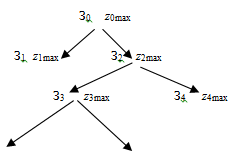
\includegraphics{pictures/picturefile_5_1.png}}
\caption*{Рис. 5.1. Схема метода ветвей и границ}
\label{picture_5_1}
\end{figure}

Вычисления заканчиваются после того, когда все очередные задачи окажутся прозондированными. Если решается задача на максимум, то среди всех разрешимых прозондированных задач выбирается та, у которой самое большое значение z$_{max}$. Эта задача и дает точку максимума исходной задачи.

Метод ветвей и границ является универсальным методом, применимым как к полностью целочисленным задачам, так и к частично целочисленным, и даже к произвольным задачам дискретного программирования. Коммерческие задачи обычно решаются этим методом. В некоторых случаях, однако, этот метод трудно реализовать из-за большого объема машинного счета.

Следует отметить, что большинство типов задач дискретного программирования имеют экспоненциальную сложность (см. п. 1.7). Исключение составляют задача о назначениях, задача о ранце с булевыми переменными и некоторые другие, имеющие полиномиальную сложность. Таким образом, при больших размерностях большинство задач дискретного программирования за разумное время решить нельзя.
\\

\addcontentsline{toc}{subsection}{Контрольные вопросы и задачи для самостоятельного решения}
\subsection*{Контрольные вопросы и задачи для самостоятельного решения}

\begin{enumerate}
	\item{Какие задачи называют задачами линейного целочисленного (частично целочисленного, дискретного, частично дискретного) программирования?}
  \item{Сформулируйте задачу о назначениях. В чем заключается связь между задачей о назначениях и транспортной задачей?}
  \item{Сформулируйте задачу о ранце.}
  \item{В чем заключается основная идея методов отсечений? Опишите первый алгоритм Гомори для полностью целочисленных задач.}
  \item{Как строится сечение Гомори второго рода?}
  \item{Какова роль двойственного симплекс метода (метода последовательного уточнения оценок) при применении сечений Гомори первого и второго рода?}
  \item{В чем заключается метод ветвей и границ?}
  \item{то можно сказать о сложности задач дискретного программирования?}
\end{enumerate}

\textit{Решить задачи о назначениях 5.1, 5.2.}


\zadanie{
Имеется пять механизмов и пять видов работ, которые этими механизмами могут выполняться. Матрица эффективностей имеет вид
$$
\begin{pmatrix}
2 & 3 & 3 & 5 & 4\\
4 & 2 & 4 & 6 & 2\\
2 & 2 & 2 & 4 & 3\\
4 & 3 & 4 & 3 & 5\\
0 & 1 & 0 & 3 & 0\\
\end{pmatrix}.
$$

Найти оптимальное распределение механизмов по видам работ.

{\bfОтвет:} Первый механизм назначается на пятую работу, второй — на четвертую, третий — на первую, четвертый — на третью, пятый — на вторую.}

\zadanie{
Для выполнения четырех видов землеройных работ используются четыре экскаватора четырех различных типов. Производительность экскаватора i-ого типа при выполнении j-ой работы задается матрицей
$$
\begin{pmatrix}
0,9 & 0,6 & 0,7 & 0,9 \\
0,7 & 0,8 & 0,9 & 0,8 \\
0,8 & 0,6 & 0,8 & 0,9 \\
0,8 & 0,7 & 0,9 & 0,7
\end{pmatrix}.
$$

Найти такое распределение экскаваторов по видам работ, которое обеспечивает максимальную производительность.

{\bfОтвет:} Экскаватор первого типа следует назначить на первый вид работ, второго типа — на второй, третьего типа — на четвертый и четвертого типа — на третий вид работ.\\}

\textit{С помощью графического истолкования найти решения задач целочисленного программирования 5.3 — 5.5.}
\zadanie{
\begin{center}
$z = x_1+x_2 \rightarrow max,$
$$
\begin{cases}
   x_1 + x_2 \leq 7,\\
   4x_1 - 5x_2 \leq 5,\\
   2x_1 + 11x_2 \leq 38;
\end{cases}
$$
$x_1 \geq 0, x_2 \geq 0,\ \  x_1,x_2 -$ целые
\end{center}

{\bfОтвет}: z$_{max}=5$; точек максимума две: M(3,2) и N(2,3).}

\zadanie{
\begin{center}
$z = 3x_1+x_2 \rightarrow min,$
$$
\begin{cases}
   -4x_1 + x_2 \leq 29,\\
   3x_1 - x_2 \leq 15,\\
   5x_1 + 2x_2 \geq 38;
\end{cases}
$$
$x_1,x_2 \geq 0,\  x_1,x_2 -$ целые
\end{center}

{\bfОтвет}: z$_{min}=19$; точка минимума (0;19).}

\zadanie{
\begin{center}
$z = 5x_1+7x_2 \rightarrow min,$
$$
\begin{cases}
   -3x_1 + 14x_2 \leq 78,\\
   5x_1 - 6x_2 \leq 26,\\
   x_1 + 4x_2 \geq 25;
\end{cases}
$$
$x_1,x_2 \geq 0,\  x_1,x_2 -$ целые
\end{center}

{\bfОтвет}: z$_{min}=52$; точка минимума (2; 6).\\}

\textit{Пользуясь алгоритмами Гомори найти решения задач 5.6 — 5.10.}
\zadanie{
\begin{center}
$z = 2x_1+x_2 \rightarrow max;$
$$
\begin{cases}
   6x_1 +4x_2 +x_3 = 24,\\
   3x_1 - 3x_2 + x_4 = 9,\\
   -x_1 + 3x_2 + x_5 = 3;
\end{cases}
$$
$x_i \geq 0, \ \ x_i -$ целые($i = \overline{1,5}$).
\end{center}

{\bfОтвет}: z$_{max}=7$; точка максимума (3; 1; 2; 3; 3).\\}

\zadanie{
\begin{center}
$z = 3x_1+2x_2 \rightarrow max;$
$$
\begin{cases}
   x_1 +x_2 +x_3 = 13,\\
   x_1 - x_2 + x_4 = 6,\\
   -3x_1 + x_2 + x_5 = 9;
\end{cases}
$$
$x_i \geq 0, \ \ x_i -$ целые($i = \overline{1,5}$).
\end{center}

{\bfОтвет}: z$_{max}=35$; точка максимума (9; 4; 0; 1; 32).\\}

\zadanie{
\begin{center}
$z = 7x_1+x_2 \rightarrow max;$
$$
\begin{cases}
   9x_1 + 4x_2 +x_3 = 110,\\
   11x_1 - 3x_2 + x_4 = 24,\\
   2x_1 - 7_2 + x_5 = 15;
\end{cases}
$$
$x_i \geq 0, \ \ x_i -$ целые($i = \overline{1,5}$).
\end{center}

{\bfОтвет}: z$_{max}=84$; точка максимума (12; 0; 2; 108; 9).\\}

\zadanie{
\begin{flushleft}
\ \ \ \ \ $z = 60x_1+70x_2 + 120,4x_3 +130x_4  \rightarrow max;$
$$
\begin{cases}
   x_1 + x_2 + x_3 + x_4= 16,\\
   x_1 + 1,85x_2 +  x_3 + x_4 \leq 16,\\
    4x_1 + 6,9x_2 + 10x_3 + 13x_4 \leq 100,\\
   6,3x_1 + 5x_2 + 4x_3 + 3x_4 \leq 100,\\
    x_1 + x_2 + x_3 + x_4 \geq 10;
\end{cases}
$$
\ \ \ \ \ $x_i \geq 0, \ \ x_i -$ целые($i = 1,4$).
\end{flushleft}

{\bfОтвет}: z$_{max}=1322,4$; точка максимума (10; 0; 6; 0).\\}

\zadanie{
\begin{flushleft}
\ \ \ \ \ $z = 5x_1+2x_2 - 3x_3 +2x_4 +3x_5 -3x_6 \rightarrow max.$
$$
\begin{cases}
   5x_1 + 6x_2 + 4x_3 + 2x_4 - 3x_5 + 5x_6= 11,\\
   5x_1 + 5x_2 +  7x_3 + 3x_5 + 5x_6= 10,\\
   2x_1 +2 x_2 + 2x_3 + 3x_5 = 4;
\end{cases}
$$
\ \ \ \ \ $x_i \geq 0, \ \ x_i -$ целые($i = \overline{1,6}$).
\end{flushleft}

{\bfОтвет}: z$_{max}=7$; точка максимума (1; 1; 0; 0; 0; 0).}
